\documentclass[a4paper,amsmath]{oblivoir}

\usepackage{fapapersize}
\usefapapersize{*,*,1in,*,1in,*}

\makeatletter
\let\ATonum\@onum
\makeatother

\usepackage{esgutil}


\usepackage{xcolor}
\usepackage{graphicx}
\usepackage{hologo}
\usepackage{relsize}
\usepackage{tcolorbox}
\tcbuselibrary{listings,breakable}
\tcbset{listing engine=listings,colframe=cyan,colback=cyan!5!white}

\setmainfont{TeX Gyre Pagella}
\setsansfont{Noto Sans}
\setmonofont{Noto Sans Mono}
\setkomainfont(Noto Serif CJK KR)(* Bold)(Noto Sans CJK KR)
\setkosansfont[Noto Sans CJK KR]()( Bold)( Medium)
\usepackage{unicode-math}
\setmathfont{texgyrepagella-math.otf}

\newcounter{sub}
\newcommand\bangotsuite{\stepcounter{sub}\thesub}

\usepackage{tikz}
\newcommand\tikzlogo{Ti\textit{k}Z}

\setlength{\parindent}{0mm}

\newcommand\pkg[1]{\textsf{#1}}

\ExplSyntaxOn 

\NewDocumentEnvironment {intro} {o}
{
    \IfValueTF { #1 }
    {
        \int_set:Nn \l_tmpa_int { #1 }
    }
    {
        \int_set:Nn \l_tmpa_int { 1 }
    }
    \noindent \rule {\linewidth}{3pt}
    \par 
    \sffamily [No.\space\int_use:N \l_tmpa_int ]\ \ 
    \bfseries
}
{
    \hfill \underline{\hphantom{2019}}년~\underline{\hphantom{06}}월~ \underline{\hphantom{25}}일 
    \par 
    \vskip -.3\baselineskip 
    \noindent \rule {\linewidth }{1pt}
    \par 
    \vskip .5\baselineskip 
}

\NewDocumentCommand \exverb { d|| }
{
    \texttt { \tl_to_str:n { #1 } }
}

\ExplSyntaxOff 

\NewDocumentEnvironment {questiona} { m }
{
%    \medskip
    \begin{tcolorbox}[title={#1},fonttitle={\sffamily\bfseries}]
}{%
    \end{tcolorbox}
}

\NewDocumentEnvironment {questionp} { }
{
%    \medskip
    \begin{tcolorbox}[colframe=orange!30!black!60,colbacktitle=orange!25!gray,
    title={연습문제},fonttitle={\sffamily\bfseries}]
}{%
    \end{tcolorbox}
}


\NewDocumentEnvironment {exampleonly} {}
{%
%    \begin{tcblisting}{listing only}
    \expandafter\tcblisting{listing only,breakable,before={\par\medskip\setstretch{1}}}
}{
    \endtcblisting
%    \end{tcblisting}
}

\NewDocumentEnvironment {exampleside} {}
{%
    \tcblisting{listing side text,breakable,before={\par\medskip\setstretch{1}}}%
}{%
    \endtcblisting
}

%\NewDocumentEnvironment {examplebelow} {}
%{%
%    \medskip
%    \tcblisting{text below listing,breakable}%
%}{%
%    \endtcblisting
%}
\newtcblisting{examplebelow}{breakable,before={\par\medskip\setstretch{1}}}

\begin{document}

\begin{intro}[4]
Flame of Passion
\end{intro}

\begin{questiona}{문제}
인자로 주어지는 정수 이하의 모든 소수를 출력하는 명령 \verb|\primes|를 작성하여라.
\tcblower
입력: \verb|\primes{10}| \\
출력: 2, 3, 5, 7
\end{questiona}

다음과 같은 방법으로 소수를 구하자.

\medskip

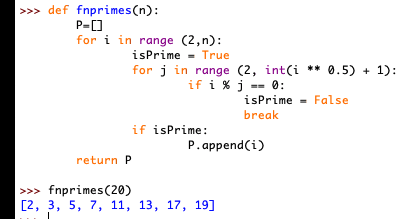
\includegraphics[scale=.8]{Screenshot-1}


\section{\textsf{fp} 연산}

\TeX 과 \LaTeX 에 있는 “수”는 count와 dimension뿐이다. expl3는 fp 자료형을 도입하여 \TeX 에 현저히 부족한 실수 계산을 보완하려 하였다.

\medskip

\hangfrom{붙임 \bangotsuite: }expl3가 처음 작성되기 시작하던 무렵에는 \textsf{pgf}의 계산 엔진을 활용하였다. 현재는 그렇지 않으나 이런 까닭에 \textsf{pgfmath}와 유사한 데가 남아 있다.

\hangfrom{붙임 \bangotsuite: }\textsf{pgfmath} 등장 이전에는 실수 계산을 위한 패키지들이 존재하였다. \texttt{realcalc}, \texttt{fp} 등이 이에 해당한다. 

\hangfrom{붙임 \bangotsuite: }expl3의 fp는 유효숫자(significand) 16자리, 지수 $\pm 10000$ 범위의 수와, 부호 있는 $0$, 부호 있는 $\infty$를 포함한다.

\medskip

fp 자료형의 핵심 함수는 \verb|\fp_eval:n|이다. 인자로 주어지는 식을 parsing하여 결과를 fp형식으로 처리한다.

\begin{examplebelow}
\ExplSyntaxOn
\fp_eval:n { 10/3 }
\ExplSyntaxOff
\end{examplebelow}

중요한 연산자와 부호는 다음과 같다. 

\begin{itemize} \firmlist
\item \verb|+|, \verb|-|, \verb|*|, \verb|/|, \verb|( )|
\item \verb|e| 부동소수점 실수 표현에 사용하는 부호이며 자연로그의 밑 $e$와는 관계없다. \verb|1.666e2| =  
\ExplSyntaxOn
\fp_eval:n { 1.666e2 }

\item \verb|inf| 무한대. $+\infty$.
\item \verb|**| 지수 연산자. \verb|^|를 써도 된다고 하나 \verb|**|를 일관되게 쓰는 것을 권장한다. \verb|\fp_eval:n {2**10}| = 
\ExplSyntaxOn
\fp_eval:n {2**10}
\ExplSyntaxOff

\item \verb|&&|, \verb+||+, \verb|!| 논리 연산자 and, or, not이다. 다른 자료형에서와 달리 다음과 같은 경우도 의미를 가진다. 이 연산의 결과가 $0$인 것은 boolean FALSE인 것과 동일하다. $1$이면 TRUE이다.
\begin{examplebelow}
\ExplSyntaxOn
\fp_set:Nn \l_tmpa_fp { 2.0 }
\fp_eval:n { \l_tmpa_fp < 0.5 || \l_tmpa_fp = 2.0 }
\ExplSyntaxOff
\end{examplebelow}

\item \verb|?:| 3항 연산자이다. \verb|\fp_eval:n { A ? a : B ? b : c } | 형식으로 쓸 수 있다. if A then a elseif B then b else c fi fi의 의미를 갖는다. A, B, C는 조건 연산식이고 a, b, c는 fp 값이다. (즉 일반 매크로가 a, b, c 자리에 올 수 없다.)
C같은 언어에 익숙하다면 이 3항 연산자도 쉽게 이해할 수 있겠지만, 코드의 가독성이 떨어지기 때문에 남용하는 것은 권하지 않는다.
\begin{examplebelow}
\ExplSyntaxOn
\fp_set:Nn \l_tmpa_fp { 2.00 }
\fp_eval:n {
    \l_tmpa_fp < 0.5 ? 1.0 :
    \l_tmpa_fp ** 2 < 3 ? 2.0 : 3.0
}
\ExplSyntaxOff
\end{examplebelow}
\end{itemize}

fp 함수는 \verb|\fp_eval:n| 범위 안에서 연산할 수 있는 함수들이다.

\begin{itemize}
\item \texttt{exp, ln, fact} : $e^{\cdot}$, $\ln$, factorial.
자연로그의 밑($e$)을 나타내려면 
\begin{exampleside}
\ExplSyntaxOn
\fp_set:Nn \l_e_fp { exp(1) }
\fp_use:N \l_e_fp
\ExplSyntaxOff
\end{exampleside}

\begin{examplebelow}
\ExplSyntaxOn
$\log \c_math_subscript_token {10} 2 = \fp_eval:n { ln(2) / ln(10) } $
\ExplSyntaxOff
\end{examplebelow}

\item \texttt{sin, cos, tan, cot, csc, sec} : 호도법(radian) 각을 인자로 취한다.
\item \texttt{sind, cosd, tand, cotd, cscd, secd} : 도(degree)를 인자로 취한다.

\item \texttt{sqrt} 제곱근.

\item \texttt{pi} : $\pi \simeq \ExplSyntaxOn
\fp_eval:n { pi }
\ExplSyntaxOff
$.

\item \texttt{round, trunc} 반올림 또는 버림. 

\begin{exampleside}
\ExplSyntaxOn
\fp_eval:n { round ( 3.14159 ) } \par
\fp_eval:n { round ( 3.14159, 3 ) }
\ExplSyntaxOff
\end{exampleside}

\item \texttt{ceil, floor} 

\end{itemize}

\paragraph{type 변환}

\begin{enumerate}[\expandafter\ATonum1] \firmlist
\item 숫자로 이루어진 tl은 확장하여 \verb|\fp_eval:n| 하면 된다. \verb|\fp_eval:n|의 인자 영역에 들어간 한 번 또는 두 번 확장가능한 tl은 자연스럽게 확장된다.

\item 정수(int)는 \verb|\fp_eval:n| 범위 안에서 바로 쓸 수 있다.
\begin{examplebelow}
\ExplSyntaxOn
\int_set:Nn \l_tmpa_int { 2 }
\fp_eval:n { sin ( ( \l_tmpa_int ** 0.4 ) pi ) }
\ExplSyntaxOff
\end{examplebelow}

\item \verb|\fp_eval:n|의 결과의 소수부(decimal part)가 0이면 int에 자연스럽게 할당된다.

\item \verb|floor, ceil| 연산의 결과는 int에 할당된다.

\item 일반적인 fp는 \verb|trunc 0| 하거나 \verb|round 0|하면 int에 할당된다.

\begin{exampleside}
\ExplSyntaxOn
\int_set:Nn \l_tmpa_int { \fp_eval:n { 6/3 } } 
\int_use:N \l_tmpa_int \par
\int_set:Nn \l_tmpa_int { \fp_eval:n { ceil ( 3/2 ) } }
\int_use:N \l_tmpa_int \par 
\int_set:Nn \l_tmpa_int { \fp_eval:n { trunc ( 100 * sind ( 20 ) ) } }
\int_use:N \l_tmpa_int 
\ExplSyntaxOff

\end{exampleside}
\end{enumerate}

길이(dim)와 fp의 관계는 아주 중요하므로 dim을 다루는 곳에서 자세히 연습하기로 한다.



\bigskip

이제 다음 문제를 풀어보자.

\medskip

\begin{questiona}{보조문제 1}
주어진 정수의 제곱근을 넘지 않는 최대 정수를 출력하여라.
\end{questiona}

$x$를 넘지 않는 최대 정수를 $\lfloor x \rfloor$로 나타내기로 하면, 
\begin{exampleside}
\ExplSyntaxOn
$\lfloor 2.95 \rfloor = \fp_eval:n { floor ( 2.95 ) } $
\ExplSyntaxOff
\end{exampleside}
이다. 또는 인자 없이 trunc하여도 같다. 이 때 truncate가 소수점 위치에서 일어나기 때문이다. 

\begin{examplebelow}
\ExplSyntaxOn

\cs_new:Npn \get_floor_sqrt:n #1
{
    \fp_eval:n { floor ( sqrt ( #1 ) ) }
}

\get_floor_sqrt:n { 20 }

\ExplSyntaxOff
\end{examplebelow}

\section{cs와 인자 확장}

우리는 지금까지 함수를 정의하는 데 \verb|\cs_new:Npn|을 사용해왔다. 이제 \verb|\cs_set:Npn|을 소개하려 하는데, 이 명령은 몇 가지 용법을 가지고 있다.

\begin{enumerate}[(1)] \firmlist
\item 이미 정의된 함수(cs)의 내용을 수정할 때. 실제로는 \verb|\cs_new:Npn| 하지 않아도 바로 \verb|\cs_set:Npn|할 수 있는데 그렇게 하지 않도록 유도하는 이유는 \hologo{plainTeX}의 \verb|\def| 위험성과 같은 이유에서이다. 즉 그 함수가 이미 정의되어 있는지를 체크하지 않기 때문에 발생하는 위험을 줄이기 위해서 \verb|\cs_new|를 쓰도록 한 것이다.
\item 함수(즉 \verb|:|와 인자형 지시자를 반드시 갖는 cs) 이름만이 아니라 일반 매크로의 내용을 정의하려 할 때

\item 지역적으로(locally) 함수의 동작을 잠시 바꾸려 할 때. 그룹 안에서 \verb|\cs_set:N|한 것은 그룹을 벗어나면 효력을 잃는다.
\end{enumerate}

다음에 예를 들어본다.

\begin{exampleside}
\ExplSyntaxOn
\cs_new:Npn \foo_fn:n #1 { This~is~#1 }
\foo_fn:n { test }
\par
\cs_set:Npn \foo_fn:n #1 { You~are~#1 }
\foo_fn:n { beautiful }
\ExplSyntaxOff
\end{exampleside}

\begin{exampleside}
\ExplSyntaxOn
\cs_set:Npn \mytest #1 { Hello,~#1! }
\mytest{boys}
\ExplSyntaxOff
\end{exampleside}

이 두 번째 사용법을 이용하면 \verb|\NewDocumentCommand|를 쓰지 않더라도 문서 명령을 만들 수 있다. 즉
\begin{examplebelow}
\ExplSyntaxOn
\cs_set_eq:NN \hello \foo_fn:n
\ExplSyntaxOff
\hello{nice}
\end{examplebelow}

이와 같이 정의할 수 있는 것이다. 

일반적인 \LaTeX{} 명령은 “풀리지 않게” 정의하는 것이 책갈피나 moving arguments에서 깨지지 않게 보호할 수 있다. 그렇기 때문에 사용자 문서 명령은 \verb|\NewDocumentCommand|를 쓰는 것이 바람직하다.
그렇지만 아주 특별히, 풀리는 명령을 정의해야 할 필요가 있을 때, 그것도 문서 명령 비슷하게 해야 할 때 이것이 한 가지 팁이 될 수 있다. (그러나 \verb|\cs_if_...| 명령으로 이렇게 정의된 명령을 검사하면 에러가 발생할 가능성도 있으므로 주의를 요한다.)

\bigskip

cs를 정의할 때 인자를 확장하려면 어떻게 하는가? 예를 들어 \verb|\foo_fn:o|라는 형태로, 즉 들어오는 인자를 무조건 한 번 확장하여 사용하려 한다면 다음과 같이 정의한다.

\begin{exampleonly}
\ExplSyntaxOn
\cs_new:Npn \foo_a:n #1
{
    \fbox{#1}
}

\cs_generate_variant:Nn \foo_a:n { V, o }
\ExplSyntaxOff
\end{exampleonly}

\verb|\cs_generate_variant:Nn|은 모든 확장형을 다 쓸 수 있게 해주는 것은 아니다. 여기서는 다음 사항을 기억하자.

\begin{enumerate}[(1)] \firmlist
\item 인자가 tl일 때, n을 V, o, x로 확장할 수 있고, N을 V로 확장할 수 있다.
\item 인자가 int, fp, dim일 때, n을 o, x로 확장할 수 있고, N을 V로 확장할 수 있다.
\end{enumerate}

유념할 것은 예컨대 자신이 함수의 이름을 \verb|\my_func:x|라고 지었다고 해서 바로 x확장이 일어나는 것은 아니라는 것이다. 그러므로 일단 모든 인자를 무조건 n으로 하는 함수 기본 형을 정의한 후에 이의 variant를 기술하는 것이 좋은 코딩 방법이 된다.

\section{소수 구하기}

원래의 문제로 돌아와서, 주어진 알고리즘을 잘 상고해보면 \verb|break| 문이 들어 있는 것을 볼 수 있다.
그러므로 for 루프를 쓰도록 되어 있지만 우리는 map을 활용해야 한다.

$n$이 주어지면 그 수까지의 자연수를 담고 있는 clist를 먼저 만들기로 하자. 1은 제외한다.

\begin{examplebelow}
\ExplSyntaxOn

\cs_new:Npn \build_numlist:n #1
{
    \clist_clear:N \l_tmpa_clist
    \int_step_inline:nnn { 2 } { #1 }
    {
        \clist_put_right:Nn \l_tmpa_clist { ##1 }
    }
}

\build_numlist:n { 100 }
\clist_use:Nn \l_tmpa_clist { , ~ }

\ExplSyntaxOff
\end{examplebelow}

그리고, 주어진 수의 $\lfloor x \rfloor$까지의 clist도 하나 만든다.

\begin{examplebelow}
\ExplSyntaxOn

\cs_set:Npn \build_numlist:n #1
{
    \clist_clear:N \l_tmpa_clist
    \int_step_inline:nnn { 2 } { #1 }
    {
        \clist_put_right:Nn \l_tmpa_clist { ##1 }
    }
    
    \clist_clear:N \l_tmpb_clist
    \int_step_inline:nnn { 2 } { \get_floor_sqrt:n { #1 } }
    {
        \clist_put_right:Nn \l_tmpb_clist { ##1 }
    }
}

\build_numlist:n { 100 }
a~:~\clist_use:Nn \l_tmpa_clist { , ~ } \par
b~:~\clist_use:Nn \l_tmpb_clist { , ~ }

\ExplSyntaxOff
\end{examplebelow}

처음에 제시한 알고리즘을 구현하면 다음과 같다.

\begin{examplebelow}
\ExplSyntaxOn
\cs_set:Npn \get_floor_sqrt:n #1
{
    \fp_eval:n { floor ( sqrt ( #1 ) ) }
}

\cs_set:Npn \build_numlist:n #1
{
    \clist_clear:N \l_tmpa_clist
    \int_step_inline:nnn { 2 } { #1 }
    {
        \clist_put_right:Nn \l_tmpa_clist { ##1 }
    }
    
    \clist_clear:N \l_tmpb_clist
    \int_step_inline:nnn { 2 } { \get_floor_sqrt:n { #1 } }
    {
        \clist_put_right:Nn \l_tmpb_clist { ##1 }
    }
}

\cs_new:Npn \fn_primes:n #1
{
    \clist_gclear:N \g_tmpa_clist
    
    \build_numlist:n { #1 }
    
    \clist_map_inline:Nn \l_tmpa_clist
    {
        \bool_gset_true:N \g_tmpa_bool
        \int_gset:Nn \g_tmpa_int { ##1 }
        \clist_map_function:NN \l_tmpb_clist \sub_fn:n
        \bool_if:NT \g_tmpa_bool
        {
            \clist_put_right:Nn \g_tmpa_clist { ##1 }
        }
    }
    
    \clist_use:Nn \g_tmpa_clist { , ~ }
}

\cs_new:Npn \sub_fn:n #1
{
    \bool_if:nT 
    {
        \int_compare_p:n { \int_mod:nn { \g_tmpa_int } { #1 } == 0  }
        &&
        \int_compare_p:n { \g_tmpa_int != #1 }
    }
    {
        \bool_gset_false:N \g_tmpa_bool
        \clist_map_break:
    }
}

\cs_set:Npn \fnprimes #1 
{
    \fn_primes:n { #1 }
    {}~( \clist_count:N \g_tmpa_clist )
}

\ExplSyntaxOff

\fnprimes{21}

\end{examplebelow}

어찌 됐든 답을 구할 수는 있었지만 이 방법은 다음 두 가지 때문에 좋은 해결책이 못 된다.
(1) clist에 넣을 수 있는 아이템의 개수에 제한이 있다.
(2) clist 또는 seq에 정수를 입력하는 것이 효율적이지 못하다. 구하려는 수가 커지면 clist 입출력에 너무 많은 시간이 소요된다.

만약 \verb|\int_step_...|을 중간에 중단할 수 있는 break 명령이 있다면 어떻게 할 수 있을까?

\begin{examplebelow}
\ExplSyntaxOn

\cs_new:Npn \step_fn_prime:n #1
{
    \bool_gset_true:N \g_tmpa_bool
    \int_step_inline:nnn {2} { \fp_eval:n { floor ( sqrt ( #1 ) ) } }
    {
        \int_compare:nT { \int_mod:nn { #1 } { ##1 } == 0 }
        {
            \bool_gset_false:N \g_tmpa_bool
            \esg_int_step_break:
        }
    }
    
    \bool_if:NT \g_tmpa_bool
    {
        \clist_gput_right:Nn \g_tmpa_clist { #1 }
    }
}

\cs_new:Npn \fn_new_primes:n #1
{
    \clist_gclear:N \g_tmpa_clist
    
    \int_step_function:nnN {2} { #1 } \step_fn_prime:n
    
    \clist_use:Nn \g_tmpa_clist { ,~ }
}

\fn_new_primes:n { 25 }

\ExplSyntaxOff
\end{examplebelow}

이것은 처음에 제시한 python 코드를 거의 그대로 옮긴 것이다. \verb|\esg_int_step_break:|
명령은 따로 준비하였다.


\vfill

\begin{questionp}

\fbox{기본} 1. 본문의 예제는 루프를 탈출하기 위하여 \verb|\clist_map|을 활용하였다.
그런데 while do를 쓰면 clist mapping을 이용하지 않아도 루프의 탈출 조건을 
만들 수 있다. 이를 이용하여 같은 알고리즘을 구현할 수 있겠는가?

\bigskip

\fbox{발전} 2. 주어진 수가 소수인지를 검사하는 다음과 같은 알고리즘이 있다. 이를 expl3로 구현할 수 있겠는가?

\medskip

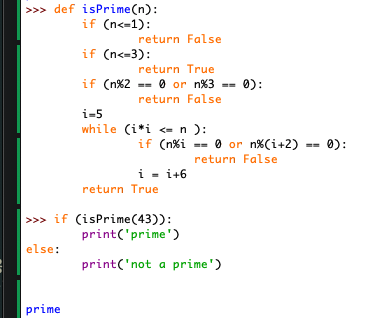
\includegraphics[scale=.78]{Screenshot-2}


\bigskip

\fbox{실력} 3. KTUG 게시판 \href{http://www.ktug.org/xe/index.php?document_srl=235888&mid=KTUG_open_board}{:235888} 글에 소인수분해 알고리즘이 소개되어 있다. 
이를 바탕으로 다음 순서로 문제를 해결하여라.
\begin{enumerate}[\ \ \expandafter\ATonum1] \firmlist
\item 두 수를 인자로 받아서 최대공약수를 구하여라.
\item 최대공약수를 소인수분해하여 결과를 clist나 seq에 저장하여라.
\item 최대공약수의 소인수를 취하여 차례로 두 수를 나누어가면서 몫(quotient)의 변화 과정을 clist나 seq에 저장하여라.
\item 준비된 세 개의 clist (seq)를 이용하여 다음 그림과 같이 출력하여라.
\end{enumerate}
\begin{center}
\begin{tabular}{r|rr}
2 & 16 & 24 \\ \cline{2-3}
2 & 8  & 12 \\ \cline{2-3}
2 & 4 & 6 \\ \cline{2-3}
  & 2 & 3 \\ 
\end{tabular}
\end{center}


\end{questionp}



\newpage

\begin{questiona}{문제}
1부터 10까지 정수의 상용로그 값을 계산하여 좌표평면에 다음 그림과 같이 나타내어라.

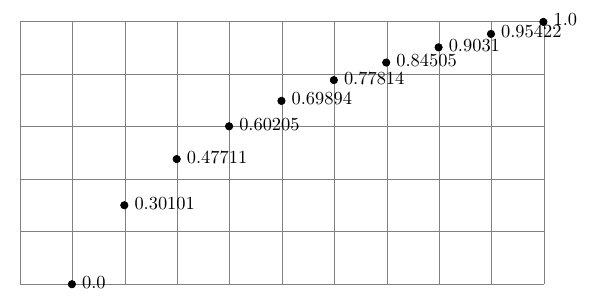
\includegraphics[width=.9\linewidth]{Screenshot-3}

\end{questiona}

먼저, 1부터 10까지 정수의 상용로그 값을 도표로 작성해보자.

\begin{exampleside}
\ExplSyntaxOn
\int_step_inline:nn { 10 }
{
    #1:~\fp_eval:n { ln ( #1 ) / ln ( 10 ) } \par
}
\ExplSyntaxOff
\end{exampleside}

소수 네째자리까지만 표현하고 싶어서 \verb|round| 함수를 써보면 다음처럼 된다.
\verb|round (0.30102999, 4)|와 같이 round할 위치를 \verb|,4|로 이어 지시해야 하는 것에 주의한다.

\begin{exampleside}
\ExplSyntaxOn
\int_step_inline:nn { 10 }
{
    #1:~\fp_eval:n { round ( ln ( #1 ) / ln ( 10 ) , 4) } \par
}
\ExplSyntaxOff
\end{exampleside}

반올림은 원하는 자리에서 잘 일어났는데 수의 표현이 가지런하지 않다. 그 이유는 fp 표현식이 끝자리 0를 모두 제거하기 때문이다.

그래서 \verb|\format_num:n| 함수를 하나 정의하였다. 이것은 들어오는 소수의 길이를 6자리로 보고 필요한 0를 채워넣은 것이다. 

\begin{examplebelow}
\ExplSyntaxOn

\cs_new:Npn \format_num:n #1
{
    \tl_set:Nn \l_tmpa_tl { #1 }
    \str_if_in:NnF \l_tmpa_tl { . }
    {
        \tl_put_right:Nn \l_tmpa_tl { .0000 }
    }
    
    \int_compare:nT { \tl_count:N \l_tmpa_tl < 6 }
    {
        \int_step_inline:nn { 6 - \tl_count:N \l_tmpa_tl }
        {
            \tl_put_right:Nn \l_tmpa_tl { 0 }
        }
    }
    
    \l_tmpa_tl
}

\cs_generate_variant:Nn \format_num:n { V, x }

\format_num:n { 2.1 }
\ExplSyntaxOff

\end{examplebelow}

현재 정의한 \verb|\format_num:n|은 일반적인 용도에 쓸 수 없다. 왜냐하면 정수 부분이 단 한 자리인 소수만을 표현할 수 있고 소수 부분은 무조건 4자리로 맞추고 있기 때문이다. 

예컨대 \verb|\formatnum[3]{123.1}|과 같이 입력하면 \verb|123.100|으로 표현해주는 함수를 정의하는 것은 스스로 해보는 즐거움을 위하여 미루어두겠다.

1에서 10까지의 상용로그를 소수 네째자리까지 표현하는 데는 이것으로 가능하니까 여기서는 그냥 쓰도록 하였다.

\begin{examplebelow}
\ExplSyntaxOn
\cs_new:Npn \print_log_value:n #1
{
    \ensuremath{#1} \c_alignment_token
    \ensuremath{
        \format_num:x { \fp_eval:n { round ( ln (#1) / ln (10), 4 ) } }
    } 
    \tabularnewline \hline
}

\begin{tabular}{|r|c|}
\hline
$x$ & $y$ \\ \hline 
\int_step_inline:nn { 9 }
{
    \print_log_value:n { #1 }
}
\ensuremath{10} \c_alignment_token 
\ensuremath{
    \format_num:n { 1 } }
\\ \hline
\end{tabular}
\ExplSyntaxOff
\end{examplebelow}


\section{\tikzlogo 와 expl3}

현 시점에서 “그리기”의 사실상 표준인 \tikzlogo 를 expl3 syntax 범위 안에서 쓰기 위해서 다음 두 가지를 주의하여야 한다.

\begin{enumerate}[(1)] \firmlist
\item \tikzlogo{} 옵션 등에 나타나는 space를 반드시 명시적으로 (틸데로써) 입력하여야 한다. \\
\verb|\tikz[rounded~corners=3pt]|

\item 콜론 문자를 직접 입력하여서는 안 된다. 이럴 때를 위하여 \verb|\c_colon_str|이라는 string 상수가 정의되어 있다.

\item \tikzlogo{} 환경과 expl3는 서로 다른 확장 규칙을 가지고 있다. expl3로 작성된 함수가 \tikzlogo{} 환경 안에서 성공적으로 풀리지 않을 수 있다. 이럴 때에는 \tikzlogo{} 환경을 ExplSyntax 범위 밖에 두는 것을 고려해보아야 한다.

\item \tikzlogo{} 환경 내부에서 반복문을 실행해야 한다면 \verb|\foreach|를 쓰는 것이 대체로 안전하다.

\item 될 수 있으면 expl3로 행하는 계산이나 함수의 확장은 \tikzlogo{} 환경 외부에서 실행하고 결과를 expandable한 tl이나 매크로로 \tikzlogo{} 함수에 넘겨주도록 코드를 작성하는 것이 좋다.
\end{enumerate}

이 몇 가지를 주의하면 ExplSyntax 안에서 \tikzlogo 를 사용하는 것이 가능하다.

\begin{examplebelow}
\ExplSyntaxOn
\cs_new:Npn \mylog:n #1
{
    \fp_eval:n { round ( ln ( #1 ) / ln ( 10 ) , 4 ) }
}
\cs_set_eq:NN \mylog \mylog:n

\begin{tikzpicture}
\draw (0,0) grid (10,5);
\foreach \x in {1,2,...,10}
    \node at (\x, 5*\mylog{\x}) [label={\format_num:x { \mylog{\x}} }] {$\bullet$};
\end{tikzpicture}
\ExplSyntaxOff
\end{examplebelow}

\paragraph{확장 (4)}

\verb|\exp_args:| 함수는 그 이름에서 알 수 있는 바와 같이 arguments를 expand하는 데 쓰는 것이다. 그런데 arguments가 아니라 멀쩡한 매크로가 있는 자리에서 그 매크로 자체를 (\verb|\expandafter| 처럼) 확장하고자 한다면 어떻게 해야 하는가?

이럴 때 쓰는 것이 \verb|\exp_last_unbraced:| 함수이다. 예를 들어보자.

\begin{exampleonly}
\ExplSyntaxOn
\begin{tikzpicture}
\draw (0,0) -- (3,3);
\end{tikzpicture}
\ExplSyntaxOff
\end{exampleonly}

이 경우에, 선분의 끝점을 매크로로 전달하는 상황을 가정한다.
\begin{exampleonly}
\ExplSyntaxOn
\tl_set:Nn \l_tmpa_tl { [very~thick,blue] }
\cs_set:Npn \my_point:n #1 { (#1,\int_eval:n { #1+1 } ) }
\tl_set:Nx \l_tmpb_tl { (0,0) -- \my_point:n { 2 } }
\begin{tikzpicture}
\draw \l_tmpa_tl \l_tmpb_tl ;
\end{tikzpicture}
\ExplSyntaxOff
\end{exampleonly}

(이 샘플은 별도로 확장 안 해도 잘 동작하지만 설명을 위해 예를 드는 것이므로)
여기서 \verb|\l_tmpa_tl|와 \verb|\l_tmpb_tl| 매크로롤 확장하여야 할 적에 다음과 같이 한다.

\begin{examplebelow}
\ExplSyntaxOn
\tl_set:Nn \l_tmpa_tl { [very~thick,blue] }
\cs_set:Npn \my_point:n #1 { (#1,\int_eval:n { #1+1 } ) }
\tl_set:Nx \l_tmpb_tl { (0,0) -- \my_point:n { 2 } }
\begin{tikzpicture}
\exp_last_unbraced:NNx \draw \l_tmpa_tl \l_tmpb_tl ;
\end{tikzpicture}
\ExplSyntaxOff
\end{examplebelow}

요약하면, 브레이스(\verb|{}|)로 둘러싸여 전달되는 부분을 확장하려면 \verb|\exp_args:|를 쓰고
단일 매크로를 확장하려 할 때는 \verb|\exp_last_unbraced:|를 쓴다고 해도 좋다.

이미 강조한 바이지만, 예를 들어 
\begin{verbatim}
\my_func:n { \l_tmpa_tl }
\end{verbatim}
이런 상황에서 \verb|\l_tmpa_tl|이 단 한 개의 문자로 이루어져 있을 때 \verb|\my_func:n \l_tmpa_tl|라고 쓰고 싶은 유혹을 충분히 느끼겠지만 확장 관련 문제가 복잡하게 얽힐 때에 대비하여 \verb|n| 아규멘트라면 중괄호를 꼭 써주어야 한다. 


\vfill

\begin{questionp}

\fbox{기본} 1. 가로 10cm, 세로 10cm이고 상하좌우 여백이 1.5cm, 모두 30페이지를 가진 pdf 문서를 작성한다. 매 페이지마다 현재 페이지가 전체 페이지수에 대하여 몇 \%인지를 표시하고 페이지 번호가 5의 배수가 되는 때 페이지의 배면색상(background color)를 cyan으로 하여라.

\bigskip

\fbox{기본} 2. 위의 pdf 문서 각 페이지의 중앙에 반지름 3cm인 원을 그리고 진행비율(현재페이지/전체페이지)을 붉은 색으로 표시하는 progress pie를 그려라.

\bigskip

\fbox{기본} 3. 중학교 수학 교과서의 부록으로 “삼각비표”가 있다. 이 표의 일부 ($0^\circ$부터 $25^\circ$까지)를 되도록 예쁘게 작성하여라.

\bigskip

\fbox{실력} 4. 다음 그림을 그려보아라. 배경색은 별도로 지정하지 않아도 좋다.

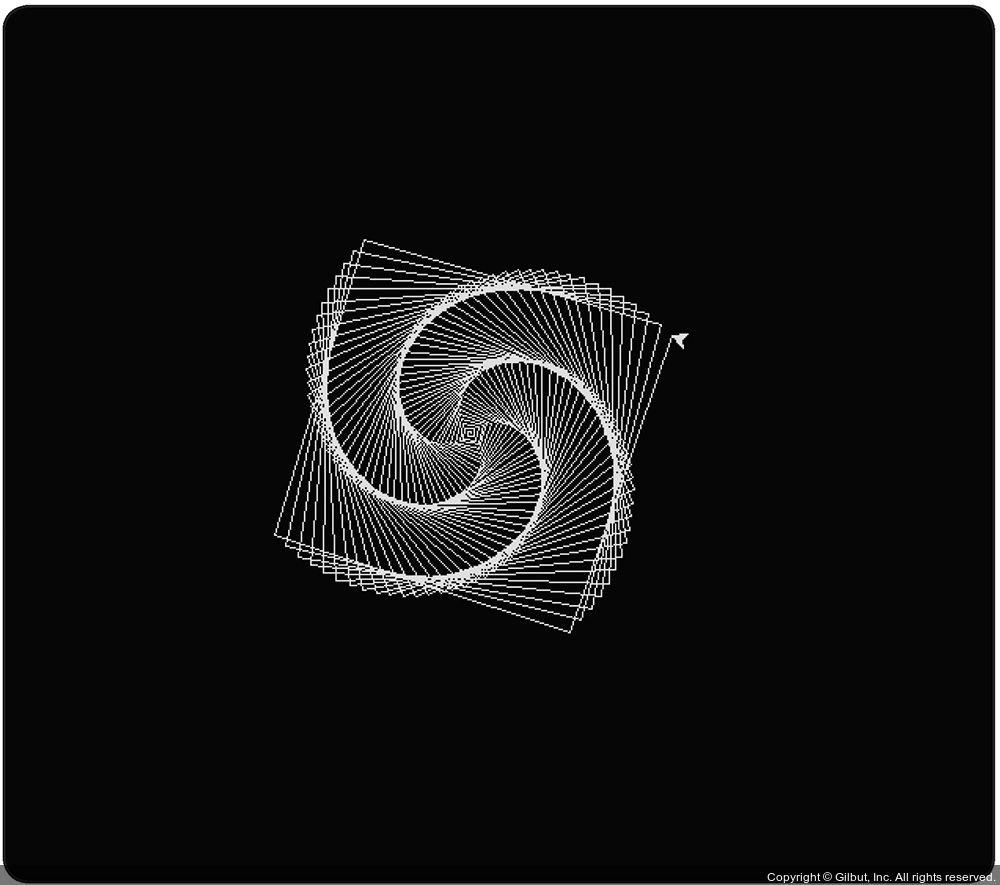
\includegraphics[width=.7\linewidth]{Screenshot-4}

\end{questionp}


\vfill
\hfill Nova de Hi.

\end{document}

